\documentclass{scrartcl}
\usepackage{mm_ws15}

\usetikzlibrary{quotes,angles,arrows,decorations.markings}


\newcommand{\sheetTitle}{Blatt 2, Abgabe 3.11.2015 12:00}
\newcommand{\FF}{\mathcal{F}}
\newcommand{\PP}{\mathcal{P}}
\newcommand{\ee}{\vec{e}}
\newcommand{\ff}{\vec{f}}

\begin{document}
\maketitle

\section{Axiome des Vektorraums \points{10}}
\label{ex:functionspace}
\begin{subex}
  \item\points{5} Sei $\FF = \{ f\colon \RR\to\RR, x \mapsto f(x) \}$ die Menge der reellen Funktionen.
  Zeigen Sie, dass $(\FF,+,\times)$ einen Vektorraum bildet, wobei Addition und Multiplikation mit einem Skalar $\lambda \in \RR$ für $f, g \in \FF$ punktweise erklärt wird
  \[
    \label{eq:operations}\tag{*}
    (f + g)(x) = f(x) + g(x), \quad (\lambda \times f)(x) = \lambda \times f(x).
  \]

  \item\points{3} Die Menge der Polynome vom Grad $n$ ist die Menge aller Funktionen, die sich als Summe der Potenzen $x^0,x^1,x^2,\dots, x^n$ der Variablen $x$ mit reellen Koeffizienten $a_0, a_1, \dots a_n$ schreiben lassen,
  \[
    \PP_n  = \left\{ f\colon \RR \to \RR, x \mapsto f(x) = \sum_{k=0}^n a_k x^k \right\}.
  \]
  Zeigen Sie, dass $(\PP_n,+,\times)$ ein Untervektorraum von $\FF$ ist.
  Hierbei sind $+$ und $\times$ wie in~\eqref{eq:operations} definiert.

  \item(4\ Zusatzpunkte) Zeigen Sie, dass die Funktionen $p_k\colon \RR \to \RR, x \mapsto x^k$ ($k=0,\ldots,n$) eine Basis für $\PP_n$ sind.
  Was schlussfolgern Sie für die Dimension von $\PP_n$?

  \item\points{2} Betrachte $\lambda \in \RR$ und $f,g \in \PP_n$ mit $f(x) = \sum_{k=0}^n a_k x^k$ und $g(x) = \sum_{k=0}^n b_k x^k$.
  Berechnen Sie explizit die Koeffizienten von $f + g$ und $\lambda \times f$ bezüglich der $p_k$.
\end{subex}

\begin{remark}{Hinweis}
  Überlegen Sie sich bei jedem Beweisschritt, welche Annahmen Sie verwenden dürfen -- Aufgaben wie~\ref{ex:functionspace}a) erscheinen ohne die nötige Sorgfalt oft trivialer als sie eigentlich sind.
  Machen Sie sich klar, dass in~\eqref{eq:operations} jeweils zwei verschiedene \quotes{$+$} und \quotes{$\times$} auf der linken und rechten Seite des Gleichheitszeichens stehen.

  Für c): Induktion nach $n$.
  Welcher Koeffizient bestimmt das Verhalten für $x \to \infty$?
  Für die präzise Formulierung benötigen Sie den Grenzwertbegriff aus der Schule oder dem Vorkurs.
\end{remark}



\section{Linearkombination und lineare Unabhängigkeit \points{8}}
Gegeben sind die Komponenten $\mat{x}$,\ldots\ von Vektoren $\vec{x}$,\ldots\ bezüglich einer Basis des $\RR^3$:
\[
  \mat{x} = \colvec{ 1 \\ 2 \\ 2 }, \quad
  \mat{y} = \colvec{ 0 \\ 1 \\ 2 }, \quad
  \mat{z} = \colvec{ -1 \\ -1 \\ 1 } \quad \textrm{und} \quad
  \mat{a} = \colvec{ 1 \\ 0 \\ 3 }, \quad
  \mat{b} = \colvec{ -5 \\ 2 \\ 1 }.
\]
\begin{subex}
   \item\points{4} Prüfen Sie, ob die Vektoren $\vec{x} , \vec{y} , \vec{z}$ linear unabhängig sind und begründen Sie, ob diese eine Basis des $\RR^3$ bilden.
   \item\points{4} Drücken Sie die Vektoren $\vec{a}, \vec{b}$ jeweils als Linearkombination von $\vec{x} , \vec{y} , \vec{z}$ aus.
 \end{subex}



\section{Komponenten eines Vektors bezüglich einer Basis \points{7}}
Gegeben seien zwei Basen $\mathcal{E} = (\ee_1, \ee_2, \ee_3)$ und $\mathcal{F} = (\ff_1,\ff_2,\ff_3)$ des dreidimensionalen Vektorraums $V$.
Damit lässt sich jedes $\vec{v} \in V$ sowohl bezüglich $\mathcal{E}$ als auch bezüglich $\mathcal{F}$ darstellen:
\[
  \label{eq:basis}\tag{+}  
  \vec{v} = v_1 \ee_1 + v_2 \ee_2 + v_3 \ee_3 = \tilde{v}_1 \ff_1 + \tilde{v}_2 \ff_2 + \tilde{v}_3 \ff_3.
\]
Die Wahl der Basis deuten wir in der Komponentenschreibweise mittels eines zusätzlichen obenstehenden Index an, d.h.
\[
  \mat{v}^\mathcal{E} = \colvec{v_1 \\ v_2 \\ v_3} \quad\mbox{und}\quad
  \mat{v}^\mathcal{F} = \colvec{\tilde{v}_1 \\ \tilde{v}_2 \\ \tilde{v}_3} 
\]
Für die Beziehung zwischen den beiden Basen gilt
\[
  \ff_1 = 2 \ee_1 + \ee_2 - \ee_3, \quad 
  \ff_2 = \ee_1 + \ee_3, \quad
  \ff_3 = -\ee_1 + \ee_2.
\]

\begin{subex}
  \item\points{4} Geben Sie die Komponenten $\mat{e}_i^\mathcal{E}$ der Basisvektoren $\ee_i$ ($i=1,2,3$) sowie die Komponenten $\mat{f}_i^\mathcal{E}$ der Basisvektoren $\ff_i$ ($i=1,2,3$) bezüglich der Basis $\mathcal{E}$ an.
  \item\points{3} Drücken Sie die Komponenten eines beliebigen Vektors $\mat{v}^\mathcal{E}$ mithilfe der Komponenten $\mat{v}^\mathcal{F}$ aus.
  Mit anderen Worten: angenommen Sie kennen die Komponenten $\tilde{v}_i$ in~\eqref{eq:basis}, finden Sie die zugehörigen Komponenten $v_i$. 
\end{subex}

\section{Kräftezerlegung \points{5}}
Eine Kugel mit Masse $m$ rollt eine geneigte Ebene mit Steigungswinkel $\varphi$ hinab.
Es wirkt die Gewichtskraft $F_\mathrm{G} = m \times g$, wobei $g$ die Fallbeschleunigung bezeichnet (die Richtung der Gewichtskraft entnehmen Sie bitte der Skizze).
Berechnen Sie daraus die Kraft $\vec{F}_\parallel$, die entlang der Bewegungsrichtung wirkt, und die Kraft $\vec{F}_\perp$, die senkrecht auf die Auflage wirkt.


\begin{center}
  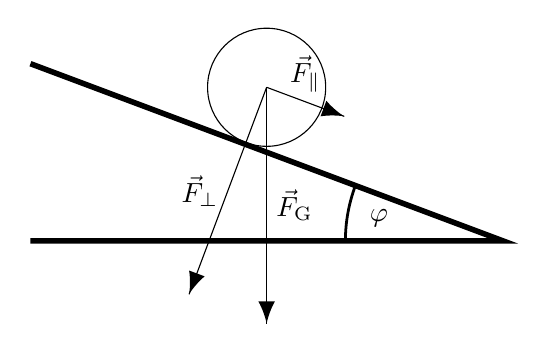
\begin{tikzpicture}[
    scale=1.5,
    myarrow/.style={decoration={markings,mark=at position 1 with %
    {\arrow[scale=2,>=latex]{>}}},postaction={decorate}},
    baseline/.style={line width=2pt}
  ]

     \draw[baseline]
      (-4,1.5) coordinate (a) node[right] {}
        -- (0,0) coordinate (b) node[left] {}
        -- (-4,0) coordinate (c) node[above right] {}
        pic["$\varphi$",draw,angle eccentricity=0.8,angle radius=2cm,line width=1pt] {angle=a--b--c};

      \coordinate (center) at (-2., 1.3) {};
      \draw (center) circle (.5);
      \draw[myarrow] (center) -- node[above] {$\vec F_\parallel$} ++ (.657, -.246); 
      \draw[myarrow] (center) -- node[right] {$\vec F_\mathrm{G}$} ++ (0,-2); 
      \draw[myarrow] (center) -- node[left] {$\vec F_\perp$} ++ (-0.657,-1.753); 


  \end{tikzpicture}
\end{center}
\end{document}
